\begin{surferPage}[Quartique de Kummer]{La Quartique de Kummer}
    En 1875, Eduard Kummer fut la première personne à se demander explicitement
    quel est le nombre maximal $\mu(d)$ de singularités d'une surface de degré
    $d$, 
    dans le cas des surfaces de degré $4$, appelées \emph{quartiques}. 
  
  Il prouva l'égalité $\mu(4)=16$. Il étudia ensuite en détail les quartiques ayant $16$
    singularités.
    Une famille particulièrement belle de ces surfaces est donnée par :
    \[\bigl(x^2+y^2+z^2-\mu^2\bigr)^2 - \lambda
    \,y_0\,y_1\,y_2\,y_3,\]
    où $\mu$ est un paramètre libre, et 
    $\lambda = \frac{3\mu^2-1}{3-\mu^2}$; les $y_i$ décrivent les côtés d'un
    tétraèdre régulier {\small
    $y_0=1-z-\sqrt{2}x$, \  
    $y_1=1-z+\sqrt{2}x$, \ 
    $y_2=1+z+\sqrt{2}y$, \ 
    $y_3=1+z-\sqrt{2}y$}
  afin de rendre la surface symétrique.
  Si la plupart des membres de cette famille ont exactement $16$ singularités réelles, 
  ce n'est pas le cas de tous :
  \begin{center}
    \vspace*{-0.2cm}\hspace*{-0.2cm}
    \begin{tabular}{@{}c@{\,}c@{\,}c@{\,}c@{\,}c@{}}
      \begin{tabular}{@{}c@{}}
        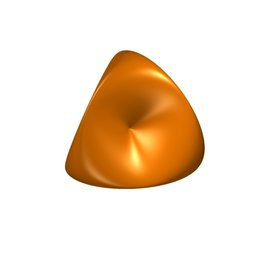
\includegraphics[height=1.4cm]{kummer_0}
      \end{tabular}
      &
      \begin{tabular}{@{}c@{}}
        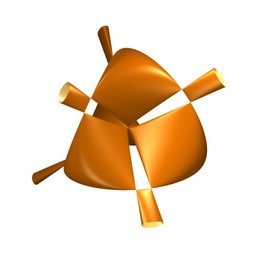
\includegraphics[height=1.4cm]{kummer_1}
      \end{tabular}
      &
      \begin{tabular}{@{}c@{}}
        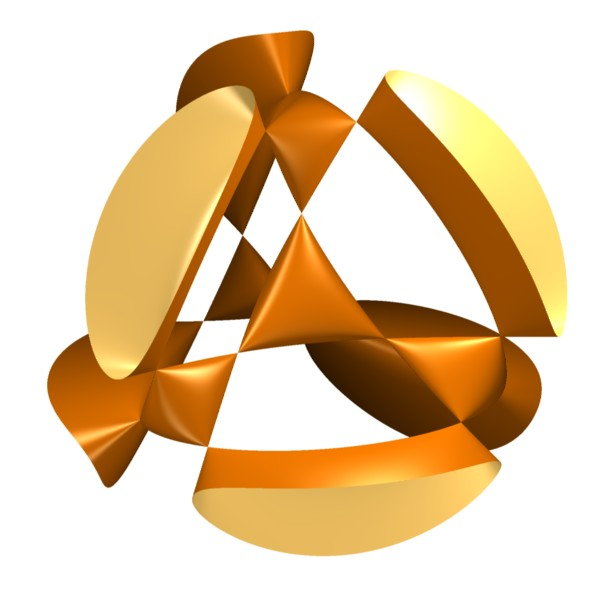
\includegraphics[height=1.4cm]{kummer_2}
      \end{tabular}
      &
      \begin{tabular}{@{}c@{}}
        
\includegraphics[height=1.4cm]{kummer_3}
      \end{tabular}
    \end{tabular}
  \end{center}
  \vspace{-0.2cm}  
   Pour des valeurs particulières des paramètres, plusieurs singularités peuvent
  être confondues.
\end{surferPage}
